\newcommand{\teorema}[2]{\begin{theorem}{#1}{th} \textbf{Demonstração.}\\ #2 \qed \end{theorem}}
\newcommand{\corolario}[2]{\begin{coro}{#1}{cr} \textbf{Demonstração.}\\ #2 \qed \end{coro}}
\newcommand{\lema}[2]{\begin{lemma}{#1}{lm} \textbf{Demonstração.}\\ #2 \qed \end{lemma}}
\newcommand{\definicao}[2]{\begin{define}{#1}{lm}  #2 \end{define}}
\newcommand{\problema}[3]{\begin{problem}{#1}{lm} \textbf{Entrada:}  \textit{#2} \\ \textbf{Questão:} #3  \end{problem}}
\newpage

\hypertarget{seuxe7uxe3o}{%
\section{Seção}\label{seuxe7uxe3o}}

Começa aqui então\ldots{}

\hypertarget{subseuxe7uxe3o}{%
\subsection{Subseção}\label{subseuxe7uxe3o}}

\hypertarget{subsubseuxe7uxe3o}{%
\subsubsection{Subsubseção}\label{subsubseuxe7uxe3o}}

Essa é a maior profundidade para seções numeradas

\hypertarget{subseuxe7uxe3o-foruxe7adamente-nuxe3o-numerada}{%
\subsection*{Subseção forçadamente não
numerada}\label{subseuxe7uxe3o-foruxe7adamente-nuxe3o-numerada}}
\addcontentsline{toc}{subsection}{Subseção forçadamente não numerada}

\hypertarget{formatauxe7uxe3o}{%
\section{Formatação}\label{formatauxe7uxe3o}}

\hypertarget{texto}{%
\subsection{Texto}\label{texto}}

Isso é \emph{italico}, e isso \textbf{negrito}; Assim é it\emph{áli}co
no meio da palavra. Assim é \texttt{monoespaçada}, e assim
\sout{riscado}.

Pode escrever assim,\\
\hspace*{0.333em}\hspace*{0.333em}\hspace*{0.333em}para que mantenha a
identação.\\
~\\
\hspace*{0.333em}\hspace*{0.333em}\hspace*{0.333em}Novas linhas\\
e tal.

Usa-se o modelo do latex de \$ para input matemático.\\
\(G(V_i, E_i) \mapsto H^{abc} \quad \forall i \in \overline{AB}\)

Usa-se o dobro de \$ para destaque

\[X_{j,t,i} = \begin{cases} 1, \text{se  $j$ é $t$, na máquina $i$}. \\ 0, \text{caso contrário} \end{cases}\]

Pode usar comandos próprios de \LaTeX

\newcommand{\tuple}[1]{\langle #1 \rangle}

\(\langle a, b, c \rangle\)

Links podem ser feitos diretamente \url{https://google.com}, ou
camuflados \href{https://google.com}{assim} Referência
obscura.\footnote{Nota de rodapé explicando referência obscura.}
\newpage

\hypertarget{quoting.}{%
\subsection{\texorpdfstring{\emph{Quoting}.}{Quoting.}}\label{quoting.}}

O Quote coloca uma frase em destaque a deslocando do texto.

\begin{quote}
Aqui é uma quote
\end{quote}

ela pode ter vários parágrafos

\begin{quote}
Aqui uma quote de vários paragrafos

taran!!!
\end{quote}

e pode ter outros textos em maior destaque

\begin{quote}
Aqui uma quote

\begin{quote}
aqui uma quote aninhada
\end{quote}

volta.
\end{quote}

\hypertarget{code-block}{%
\subsection{Code block}\label{code-block}}

Aqui tem um code block; A linguagem a seguir está definida no arquivo
lang.xml e é colorida a partir do arquivo def.theme

\begin{Shaded}
\begin{Highlighting}[numbers=left,,]
\NormalTok{Function tree.Center(): Set<Vertex>}
\NormalTok{  var aux = self}
\NormalTok{  while aux.vertices.size >= 3 do}
\NormalTok{    variable leafs = aux.leafs}
\NormalTok{    aux = aux.induced(aux.vertices - leafs)}
\NormalTok{  return aux.vertices}
\end{Highlighting}
\end{Shaded}

E aqui \texttt{Function\ Sum(a,b)\ =\ a\ +\ b;} um code \emph{inline}.

\hypertarget{estruturas}{%
\section{Estruturas}\label{estruturas}}

\hypertarget{listas}{%
\subsection{Listas}\label{listas}}

\hypertarget{lista-simples}{%
\subsubsection{Lista simples}\label{lista-simples}}

\begin{itemize}
\tightlist
\item
  A
\item
  B
\item
  C
\end{itemize}

\hypertarget{lista-com-vuxe1rias-linhas}{%
\subsubsection{Lista com várias
linhas}\label{lista-com-vuxe1rias-linhas}}

\begin{itemize}
\tightlist
\item
  Começo a falar aqui\\
  termino em outra linha.
\item
  B
\end{itemize}

\hypertarget{listas-com-listas}{%
\subsubsection{Listas com Listas}\label{listas-com-listas}}

\begin{itemize}
\tightlist
\item
  fruits

  \begin{itemize}
  \tightlist
  \item
    apples

    \begin{itemize}
    \tightlist
    \item
      macintosh
    \item
      red delicious
    \end{itemize}
  \item
    pears
  \item
    peaches
  \end{itemize}
\item
  vegetables

  \begin{itemize}
  \tightlist
  \item
    broccoli
  \item
    chard
  \end{itemize}
\end{itemize}

\hypertarget{lista-numerada-padruxe3o}{%
\subsubsection{Lista numerada padrão}\label{lista-numerada-padruxe3o}}

\begin{enumerate}
\tightlist
\item
  first
\item
  second
\item
  third
\end{enumerate}

\hypertarget{lista-numerada-a-partir-de-um-nuxba}{%
\subsubsection{lista numerada a partir de um
nº}\label{lista-numerada-a-partir-de-um-nuxba}}

\begin{enumerate}
\def\labelenumi{\arabic{enumi}.}
\setcounter{enumi}{6}
\tightlist
\item
  first
\item
  second
\item
  third
\end{enumerate}

\hypertarget{lista-numerada-diferente}{%
\subsubsection{Lista numerada
diferente}\label{lista-numerada-diferente}}

\begin{enumerate}
\def\labelenumi{\roman{enumi}.}
\tightlist
\item
  first
\item
  second
\item
  third
\end{enumerate}

\begin{enumerate}
\def\labelenumi{\arabic{enumi})}
\tightlist
\item
  first
\item
  second
\item
  third
\end{enumerate}

\hypertarget{lista-rastreavel.}{%
\subsubsection{Lista rastreavel.}\label{lista-rastreavel.}}

\begin{enumerate}
\def\labelenumi{(\arabic{enumi})}
\tightlist
\item
  primeiro exemplo.
\item
  segundo exemplo.
\end{enumerate}

Explicações de exemplos

\begin{enumerate}
\def\labelenumi{(\arabic{enumi})}
\setcounter{enumi}{2}
\tightlist
\item
  terceiro exemplo.
\end{enumerate}

\hypertarget{lista-referenciavel}{%
\subsubsection{Lista referenciavel}\label{lista-referenciavel}}

\begin{enumerate}
\def\labelenumi{(\arabic{enumi})}
\setcounter{enumi}{3}
\tightlist
\item
  Primeiro.
\item
  Segundo.
\item
  Terceiro.
\end{enumerate}

Posso referenciar aqui os elementos (4),(5),(6)

\hypertarget{linhas}{%
\subsection{Linhas}\label{linhas}}

Utilizamos uma sequencia de pelo menos 3 hífens ou asteriscos para
definir uma linha.

\begin{center}\rule{0.5\linewidth}{\linethickness}\end{center}

\begin{center}\rule{0.5\linewidth}{\linethickness}\end{center}

\hypertarget{tabelas}{%
\subsection{Tabelas}\label{tabelas}}

\hypertarget{tabelas-simples}{%
\subsubsection{Tabelas simples}\label{tabelas-simples}}

As tabelas são alinhadas de acordo com a posição relativa entre o
cabeçalho e a linha separadora.

se estiver \emph{flushed} para a direita (i.e.~alinhado a última linha
separadora ele alinhará o conteudo a direita). o mesmo se repete para
esquerda e centro.

\begin{longtable}[]{@{}rlcl@{}}
\caption{Tabela simples.}\tabularnewline
\toprule
Right & Left & Center & Default\tabularnewline
\midrule
\endfirsthead
\toprule
Right & Left & Center & Default\tabularnewline
\midrule
\endhead
12 & 12 & 12 & 12\tabularnewline
123 & 123 & 123 & 123\tabularnewline
1 & 1 & 1 & 1\tabularnewline
\bottomrule
\end{longtable}

\hypertarget{tabelas-sem-cabeuxe7alho.}{%
\subsubsection{Tabelas sem cabeçalho.}\label{tabelas-sem-cabeuxe7alho.}}

Tabelas sem cabeçalho são alinhadas de acordo com a posição relativa do
primeiro elemento.

\begin{longtable}[]{@{}rlcr@{}}
\caption{Tabela sem cabeçalho.}\tabularnewline
\toprule
\endhead
12 & 12 & 12 & 12\tabularnewline
123 & 123 & 123 & 123\tabularnewline
1 & 1 & 1 & 1\tabularnewline
\bottomrule
\end{longtable}

\hypertarget{tabela-multi-linha}{%
\subsubsection{Tabela multi linha}\label{tabela-multi-linha}}

\begin{longtable}[]{@{}clrl@{}}
\caption{Tabela multi linha.}\tabularnewline
\toprule
\begin{minipage}[b]{0.15\columnwidth}\centering
Centered Header\strut
\end{minipage} & \begin{minipage}[b]{0.10\columnwidth}\raggedright
Default Aligned\strut
\end{minipage} & \begin{minipage}[b]{0.20\columnwidth}\raggedleft
Right Aligned\strut
\end{minipage} & \begin{minipage}[b]{0.32\columnwidth}\raggedright
Left Aligned\strut
\end{minipage}\tabularnewline
\midrule
\endfirsthead
\toprule
\begin{minipage}[b]{0.15\columnwidth}\centering
Centered Header\strut
\end{minipage} & \begin{minipage}[b]{0.10\columnwidth}\raggedright
Default Aligned\strut
\end{minipage} & \begin{minipage}[b]{0.20\columnwidth}\raggedleft
Right Aligned\strut
\end{minipage} & \begin{minipage}[b]{0.32\columnwidth}\raggedright
Left Aligned\strut
\end{minipage}\tabularnewline
\midrule
\endhead
\begin{minipage}[t]{0.15\columnwidth}\centering
First\strut
\end{minipage} & \begin{minipage}[t]{0.10\columnwidth}\raggedright
row\strut
\end{minipage} & \begin{minipage}[t]{0.20\columnwidth}\raggedleft
12.0\strut
\end{minipage} & \begin{minipage}[t]{0.32\columnwidth}\raggedright
Example of a row that spans multiple lines.\strut
\end{minipage}\tabularnewline
\begin{minipage}[t]{0.15\columnwidth}\centering
Second\strut
\end{minipage} & \begin{minipage}[t]{0.10\columnwidth}\raggedright
row\strut
\end{minipage} & \begin{minipage}[t]{0.20\columnwidth}\raggedleft
5.0\strut
\end{minipage} & \begin{minipage}[t]{0.32\columnwidth}\raggedright
Here's another one. Note the blank line between rows.\strut
\end{minipage}\tabularnewline
\bottomrule
\end{longtable}

\hypertarget{tabela-com-grid}{%
\subsubsection{Tabela com grid}\label{tabela-com-grid}}

\begin{longtable}[]{@{}lll@{}}
\caption{Tabela com grid.}\tabularnewline
\toprule
\begin{minipage}[b]{0.20\columnwidth}\raggedright
Fruit\strut
\end{minipage} & \begin{minipage}[b]{0.20\columnwidth}\raggedright
Price\strut
\end{minipage} & \begin{minipage}[b]{0.27\columnwidth}\raggedright
Advantages\strut
\end{minipage}\tabularnewline
\midrule
\endfirsthead
\toprule
\begin{minipage}[b]{0.20\columnwidth}\raggedright
Fruit\strut
\end{minipage} & \begin{minipage}[b]{0.20\columnwidth}\raggedright
Price\strut
\end{minipage} & \begin{minipage}[b]{0.27\columnwidth}\raggedright
Advantages\strut
\end{minipage}\tabularnewline
\midrule
\endhead
\begin{minipage}[t]{0.20\columnwidth}\raggedright
Bananas\strut
\end{minipage} & \begin{minipage}[t]{0.20\columnwidth}\raggedright
\$1.34\strut
\end{minipage} & \begin{minipage}[t]{0.27\columnwidth}\raggedright
\begin{itemize}
\tightlist
\item
  built-in wrapper
\item
  bright color
\end{itemize}\strut
\end{minipage}\tabularnewline
\begin{minipage}[t]{0.20\columnwidth}\raggedright
Oranges\strut
\end{minipage} & \begin{minipage}[t]{0.20\columnwidth}\raggedright
\$2.10\strut
\end{minipage} & \begin{minipage}[t]{0.27\columnwidth}\raggedright
\begin{itemize}
\tightlist
\item
  cures scurvy
\item
  tasty
\end{itemize}\strut
\end{minipage}\tabularnewline
\bottomrule
\end{longtable}

\newpage
\begin{problem}{Ser Fruta.}{lm} \textbf{Entrada:}  \textit{Uma parte $F$ de uma planta $P$} \\ \textbf{Questão:} $F$ é uma fruta de $P$?  \end{problem}
\begin{define}{Frutas}{lm}  
  Parte das plantas que
  $\mapsto$
  funcionam como proteção e suplemento às sementes. \end{define}
\begin{theorem}{Frutas são boas.}{th} \textbf{Demonstração.}\\ São saborosas. \qed \end{theorem}
\begin{coro}{Banana é bom.}{cr} \textbf{Demonstração.}\\ Banana é uma fruta. \qed \end{coro}
\begin{lemma}{Banana da terra é fruta.}{lm} \textbf{Demonstração.}\\ É uma banana. \qed \end{lemma}

\begin{Shaded}
\begin{Highlighting}[]
\KeywordTok{digraph} \VariableTok{graphname}\OtherTok{\{}
\CommentTok{  }\AttributeTok{rankdir}\OtherTok{=}\VariableTok{BT}\OtherTok{;}
\CommentTok{  }\KeywordTok{edge}\CommentTok{ }\OtherTok{[}\AttributeTok{style}\OtherTok{=}\StringTok{"-latex"}\CommentTok{  }\OtherTok{];}
\CommentTok{  }\KeywordTok{node}\CommentTok{ }\OtherTok{[}\AttributeTok{style}\OtherTok{=}\VariableTok{filled}\CommentTok{ }\VariableTok{texmode}\OtherTok{=}\StringTok{"math"}\CommentTok{ }\AttributeTok{shape}\OtherTok{=}\VariableTok{circle}\CommentTok{ }\AttributeTok{fillcolor}\OtherTok{=}\VariableTok{darkolivegreen2}\OtherTok{];}
\CommentTok{  }\VariableTok{b}\OtherTok{[}\VariableTok{xlabel}\OtherTok{=}\VariableTok{tchu}\OtherTok{];}
\CommentTok{  }\VariableTok{a}\CommentTok{ }\OtherTok{->}\CommentTok{ }\StringTok{"}\SpecialCharTok{\textbackslash{}\textbackslash{}}\StringTok{Pi"}\OtherTok{;}
\CommentTok{    }\VariableTok{b}\CommentTok{ -- }\VariableTok{d}\OtherTok{;}
\OtherTok{\}}
\end{Highlighting}
\end{Shaded}

\animategraphics[height=2.8in,autoplay,controls]{12}{./pandoc/imagepdf/animate_}{0}{57}

asdajksdkywiqtehfadvsdffdddd at \ref{my_lbl}

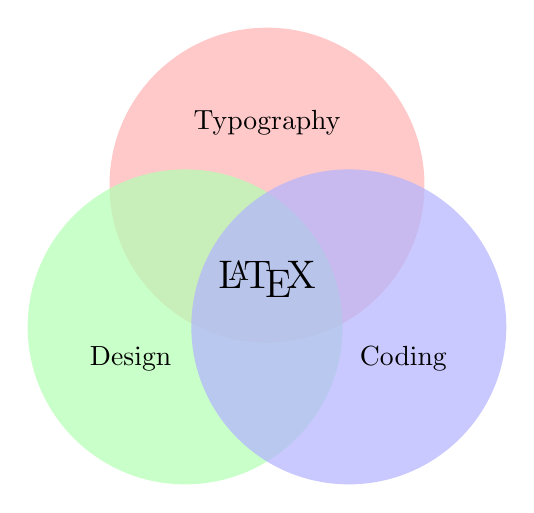
\begin{tikzpicture}
  \begin{scope}[opacity=0.7]
    \fill[red!30!white]   ( 90:1.2) circle (2);
    \fill[green!30!white] (210:1.2) circle (2);
    \fill[blue!30!white]  (330:1.2) circle (2);
  \end{scope}
  \node at ( 90:2)    {Typography};
  \node at (210:2)    {Design};
  \node at (330:2)    {Coding};
  \node [font=\Large] {\LaTeX};
\end{tikzpicture}
